\documentclass[../main.tex]{subfiles}

\begin{document}
    \section{Tujuan}
        \begin{enumerate}
            \item Memahami pengaruh letak pole terhadap tanggapan sistem
            \item Mengukur parameter-parameter tanggapan transien dan steady state
            \item Memahami serta mampu merancang kendali pole placement
        \end{enumerate}
    \section{Dasar Teori}
        Salah metode kendali yang digunakan pada sistem dengan pemodelan \textit{state space} merupakan kendali \textit{pole placement}. Metode \textit{pole placement} mengatur letak dari \textit{pole loop} tertutup, dengan memanipulasi letak pole, sistem juga dapat dimanipulasi karakteristiknya sesuai dengan penalaan yang diinginkan. Manipulasi letak \textit{pole} pada sistem  dilakukan dengan menambahkan nilai $K$ pada setiap jalur \textit{state feedback} dengan asumsi seluruh nilai veriabel \textit{state} dapat diukur dan \textit{state} pada sistem dapat dikendalikan sepenuhnya (\textit{completely state controllable}) sehingga seluruh pole pada sistem \textit{loop} tertutup dapat dipindahkan sesuai dinamika respons yang diinginkan\cite{Fahmizal}.
    \section{Hasil dan Pembahasan}
        \subsection{Latihan Soal Satu}
            \subsubsection{Konversi Pemodelan Fungsi Alih ke State Space}
                Konversi pemodelan fungsi alih ke pemodelan \textit{state space} dapat dilakukan dengan mengubah fungsi laplace kedalam bentuk \textit{canonical} sebagaimana ditunjukkan pada persamaan \eqref{persamaan_1}.
                \begin{equation}
                    \frac{Y}{U} = \frac{10}{s^3 + 6^2 + 11s + 6}
                \end{equation}
                \begin{equation}
                    \begin{split}
                        (s^3 + 6s^2 + 11s + 6) y &= 10u \\[5pt]
                        \frac{d^3y}{dt^3} + 6\frac{d^2y}{dt^2} + 11\frac{dy}{dt} + 6y &= 10u \\[5pt]
                        \dddot{y} + 6\ddot{y} + 11 \dot{y} + 6y &= 10u\\[5pt]
                        -6\ddot{y} - 11 \dot{y} - 6y + 10u &= \dddot{y}\\[5pt]
                        \label{persamaan_1}
                    \end{split}
                \end{equation}
                Dari persamaan \eqref{persamaan_1} didapatkan aturan \textit{state} ditunjukkan pada persamaan \eqref{persamaan_2}.
                \begin{equation}
                    \begin{split}
                        x_1 &= y \\[5pt]
                        x_2 &= \dot{x_1} = \dot{y} \\[5pt]
                        x_3 &= \dot{x_2} = \ddot{y}
                        \label{persamaan_2}
                    \end{split}
                \end{equation}
                Dari persamaan \eqref{persamaan_1} dan persamaan \eqref{persamaan_2} didapatkan rumus untuk state $\dot{x_3}$ ditunjukkan pada persamaan \eqref{persamaan_3}.
                \begin{equation}
                    -6x_3 - 11x_2 - 6x_1 + 10u = \dot{x_3}
                    \label{persamaan_3}
                \end{equation}
                Dari persamaan \eqref{persamaan_2} dan persamaan \eqref{persamaan_3}. didapatkan bpemodelan \textit{state space} ditunjukkan pada persamaan \eqref{persamaan_4}.
                \begin{equation}
                    \begin{split}
                        \dot{x} &= Ax +Bu \\[5pt]
                        \begin{bmatrix} \dot{x_1} \\ \dot{x_2} \\ \dot{x_3} \end{bmatrix} &= \begin{bmatrix} 0 & 1 & 0 \\ 0 & 0 & 1 \\ -6 & -11 & -6 \end{bmatrix} \begin{bmatrix} x_1 \\ x_2 \\ x_3 \end{bmatrix} + \begin{bmatrix} 0 \\ 0 \\ 1t0 \end{bmatrix} u \\[10pt]
                        y &= Cx + Du \\[5pt]
                        y &= \begin{bmatrix} 1 & 0 & 0 \end{bmatrix} \begin{bmatrix} x_1 \\ x_2 \\ x_3 \end{bmatrix}
                        \label{persamaan_4}
                    \end{split}
                \end{equation}
            \subsubsection{Controllability Test Sistem}
                tes \textit{controllability} pada sistem dilakukan menggunakan rumus sebagai berikut,
                \begin{equation} 
                    \begin{split}
                        C_m &= \begin{bmatrix} B & AB & A^{n-1}B \end{bmatrix} \\[5pt]
                        C_m &= \begin{bmatrix} B & AB & A^2B \end{bmatrix} \\[5pt]
                        \label{persamaan_5}
                    \end{split}
                \end{equation}
                elemen matriks A dan matriks B pada persamaan \eqref{persamaan_4} dimasukkan kedalam persamaan \eqref{persamaan_5} untuk mencari matriks \textit{controllability}, analisis matriks ditunjukkan pada persamaan \eqref{persamaan_6}. Dari hasil analisis yang dilakukan, diketahui sistem dalam keadaan \textit{controllable} (dapat dikendalikan) karena memiliki \textit{rank} matriks yang sama dengan \textit{state} sistem yaitu $3$.
                \begin{equation}
                    \begin{split}
                        C_m &= \left[ \begin{bmatrix} 0 \\ 0 \\ 10 \end{bmatrix} \hspace{5mm} \begin{bmatrix} 0 & 1 & 0 \\ 0 & 0 & 1 \\ -6 & 11 & -6 \end{bmatrix} \begin{bmatrix} 0 \\ 0 \\ 10 \end{bmatrix} \hspace{5mm} \begin{bmatrix} 0 & 1 & 0 \\ 0 & 0 & 1 \\ -6 & 11 & -6 \end{bmatrix}^2 \begin{bmatrix} 0 \\ 0 \\ 10 \end{bmatrix} \right] \\[5pt]
                        C_m &= \begin{bmatrix} 0 & 0 & 10 \\ 0 & 10 & -60 \\ 10 & -60 & 250\end{bmatrix}
                        \label{persamaan_6}
                    \end{split}
                \end{equation}
                Berikut merupakan program pada MATLAB yang digunakan untuk memvalidasi hasil perhitungan manual,
                \lstinputlisting[language = matlab]{assets/code/UJI_CRTB_SISTEM.m}
                Dari \textit{output} \textit{program} yang dijalankan, dapat diamati bahwa hasil analisis yang dilakukan secara matematis memiliki hasil yang sama dengan \textit{program}.
                \lstinputlisting[language = matlab]{assets/code/CONSOLE_UJI_CRTB_SISTEM.m}
            \subsubsection{Perancangan Kendali Full State Feedback}
                Sistem diketahui memiliki tiga \textit{poles} yang dituju, \textit{poles} yang dituju sebagai berikut,
                \begin{equation}
                    s = \mu_1;\mu_2;\mu_3;\cdots;\mu_n
                \end{equation}
                \begin{equation}
                    \begin{split}
                        \mu_1 &= -2 + 2\sqrt{3}i \\[5pt]
                        \mu_2 &= -2 - 2\sqrt{3}i \\[5pt]
                        \mu_3 &= -10
                    \end{split}
                \end{equation}
                Untuk menanipulasi letak \textit{pole} pada sistem, ketiga \textit{poles} saling dikalikan membentuk fungsi sebagaimana ditunjukkan pada persamaan \eqref{persamaan_7}
                \begin{equation}
                    \begin{split}
                        (s-\mu_1)(s-\mu_2)\cdots(s-\mu_n) &= 0\\[5pt]
                        \downarrow \hspace{2.5cm}&\\[5pt]
                        s^n + \alpha_1s^{n-1}+\cdots+\alpha_{n-1}s+\alpha_n &= 0
                        \label{persamaan_7}
                    \end{split}
                \end{equation}
                Perkalian antar \textit{poles} sistem membentuk fungsi sebagaimana ditunjukkan pada persamaan \eqref{persamaan_8}.
                \begin{equation}
                    \begin{split}
                        (s-(-2+2\sqrt{3}i))(s-(-2-\sqrt{3}i))(s-(-10)) &= 0\\[5pt]
                        \downarrow \hspace{3.9cm}&\\[5pt]
                        s^3 + 14s + 56s + 160 =0 \hspace{1.8cm}&\\[5pt]
                        \label{persamaan_8}
                    \end{split}
                \end{equation}
                \textit{Pole placement} merupakan metode untuk menempatkan \textit{poles} pada sistem dengan melakukan subtitusi nilai \textit{poles} yang diinginkan pada sistem. Persamaan yang digunakan pada metode \textit{pole placement} ditunjukkan pada persamaan \eqref{persamaan_9}
                \begin{equation}
                    \left| sI - (A-BK) \right| =0 \\[5pt]
                    \label{persamaan_9}
                \end{equation}
                Dari persamaan \eqref{persamaan_9} serta elemen matriks A dan B pada persamaan \eqref{persamaan_4} dilakukan analisis dengan metode \textit{pole placement} untuk mencari nilai $K$ pada sistem, ditunjukkan pada persamaan \eqref{persamaan_10} dan persamaan \eqref{persamaan_11}.
                \begin{equation}
                    \begin{split}
                        \begin{bmatrix} s & 0 & 0 \\ 0 & s & 0 \\ 0 & 0 & s \end{bmatrix} - \left( \begin{bmatrix}0 & 1 & 0 \\ 0 & 0 & 1 \\ -6 & -11 & -6\end{bmatrix} - \begin{bmatrix}0 & 0 & 0 \\ 0 & 0 & 0 \\ 10K_1 & 10K_2 & 10K_3\end{bmatrix} \right) &= 0 \\[5pt]
                        \begin{bmatrix} s & -1 & 0 \\ 0 & s & -1 \\ 0-(-6-10K_1) & 0-(-11-10K_2) & s-(-6-10K_3) \end{bmatrix} &= 0 \\[5pt]
                        \begin{bmatrix} s & 1 & 0 \\ 0 & s & 1 \\ 6+10K_1 & 11+10K_2 & s+(6+10K_3) \end{bmatrix} &= 0 \\[10pt]
                        s^3 + (6+10K_3)s^2 + (11+10K_2)s + (6+10K_1) &=0\\[5pt]
                        \label{persamaan_10}
                    \end{split}
                \end{equation}
                Dari hasil persamaan \eqref{persamaan_10} dapat dilakukan subtitusi nilai $K$ sebagai berikut,
                \begin{equation}
                    \begin{split}
                        10K_1 + 6 &= 160 \\[5pt] 
                        10K_1 &= 160 - 6 \rightarrow K_1 = 154/10 \rightarrow K_1 = 15.4 \\[10pt]
                        10K_2 + 11 &= 47 \\[5pt] 
                        10K_2 &= 56 - 11 \rightarrow K_2 = 45/10 \rightarrow K_2 = 4.5 \\[10pt]
                        10K_3 + 6 &= 14 \\[5pt] 
                        10K_3 &= 14 - 6 \rightarrow K_3 = 8/10 \rightarrow K_3 = 0.8
                        \label{persamaan_11}
                    \end{split}
                \end{equation}
                Hasil analisis nilai $K$ sistem pada persamaan \eqref{persamaan_10} dan persamaan \eqref{persamaan_11} menghasilkan nilai $K_1 = 15.4, K_2 = 4.5$ dan $K_3 = 0.8$.
            \subsubsection{Verifikasi Hasil Perancangan Kendali}
                Verifikasi hasil analisis ssecara matematis dilakukan dengan memasukkan model sistem untuk dianalisis dengan \textit{syntax} ackermann pada perangkat lunak MATLAB. Kode program untuk analisis nilai $K$ dengan \textit{syntax} ackermann sebagai berikut,
                \lstinputlisting[language = matlab]{assets/code/VALIDASI_ACKERMANN.m}
                Dari \textit{output} program, dapat diketahui bahwa hasil analisis dengan metode akcermann pada MATLAB memiliki hasil nilai $K$ yang sama dengan analisis secara matematis.
                \lstinputlisting[language = matlab]{assets/code/CONSOLE_VALIDASI_ACKERMANN.m}
            \subsubsection{Plot kendali Sistem loop tertutup}
                Kode program untuk \textit{plot} respon sistem sebagai berikut,
                \lstinputlisting[language = matlab]{assets/code/UJI_SISTEM_1.m}
                Grafik respon sistem ditunjukkan pada Gambar \ref{plot_respon_sistem_1}
                \begin{figure}[H]
                    \centering
                    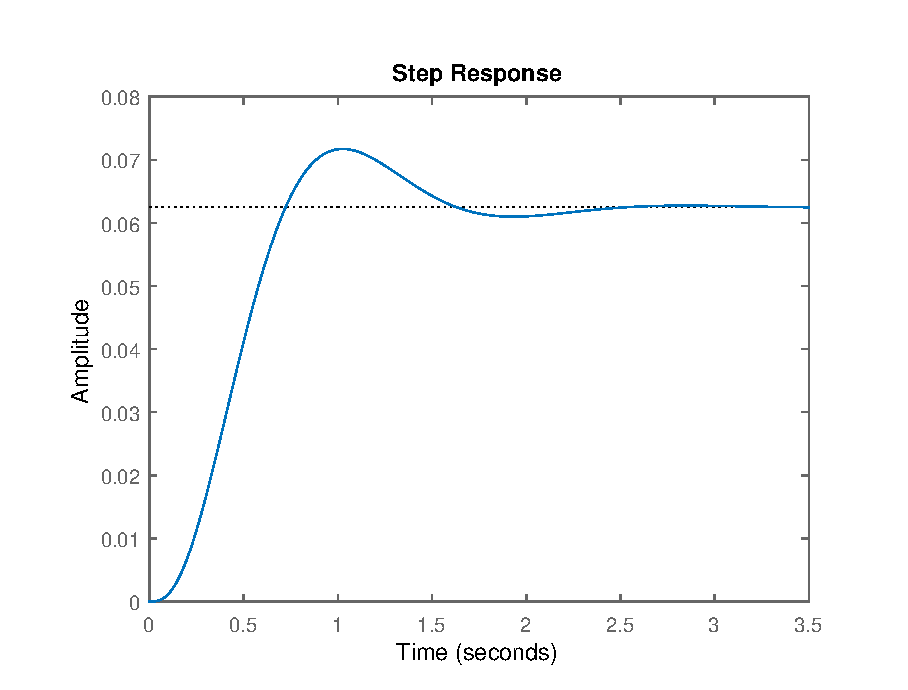
\includegraphics[width = 0.9\textwidth]{assets/image/UJI_SISTEM_1_1_rev.eps}
                    \caption{Plot respon sistem dengan \textit{input step}}
                    \label{plot_respon_sistem_1}
                \end{figure}
            \subsubsection{Perbandingan Performa Sistem}
                Perbandingan performa sistem dilakukan dengan membandingkan karakteristik sistem pada keadaan sebelum dan sesudah dilakukan \textit{tuning}. Kode program untuk perbandingan performa sistem sebagai berikut,
                \lstinputlisting[language = matlab]{assets/code/UJI_SISTEM_2.m}
                \textit{Output console} dari kode program diatas sebagai berikut, 
                \lstinputlisting[language = matlab]{assets/code/CONSOLE_UJI_SISTEM_2.m}
                Dari hasil pengamatan terhadap hasil pada \textit{output console} dan grafik pada Gambar \ref{plot_respon_sistem_2}. Sistem yang telah dilakukan \textit{tuning} memiliki nilai \textit{rise time}, \textit{settling time}, \textit{peak} serta \textit{peak time} yang lebih kecil daripada sistem sebelum dilakukan \textit{tuning}. Namun, sistem yang telah dilakukan tuning memiliki persentase \textit{overshoot} yang lebih besar daripada sistem yang belum dilakukan \textit{tuning}.
                \begin{figure}[H]
                    \centering
                    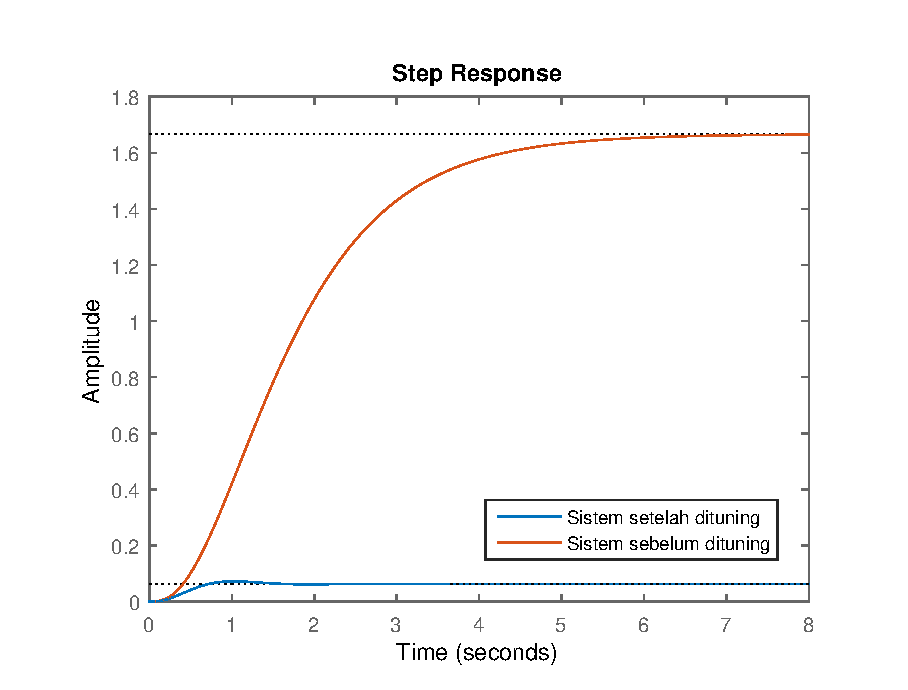
\includegraphics[width = 0.9\textwidth]{assets/image/UJI_SISTEM_1_2_rev.eps}
                    \caption{Perbandingan Respon sistem sebelum dan setelah dilakukan \textit{tuning}}
                    \label{plot_respon_sistem_2}
                \end{figure}
            \subsection{Latihan Soal 2}
                \subsubsection{Fungsi Transfer Open Loop Sistem}
                    Fungsi alih dari pemodelan kendali kecepatan motor DC ditunjukkan pada persamaan \ref{persamaan_12}
                    \begin{equation}
                        \frac{\Omega}{E_a} = \frac{K_{TM}}{JL_as^2 + (R_aJ + BL_a)s + (R_aB + K_{TM}K_M)}
                        \label{persamaan_12}
                    \end{equation}
                \subsubsection{Uji Respon Sistem dengan Input Step}
                    \lstinputlisting[language = matlab]{assets/code/UJI_STEP_MOTOR.m}
                    \lstinputlisting[language = matlab]{assets/code/CONSOLE_UJI_STEP_MOTOR_1.m}
                    \begin{figure}[H]
                        \centering
                        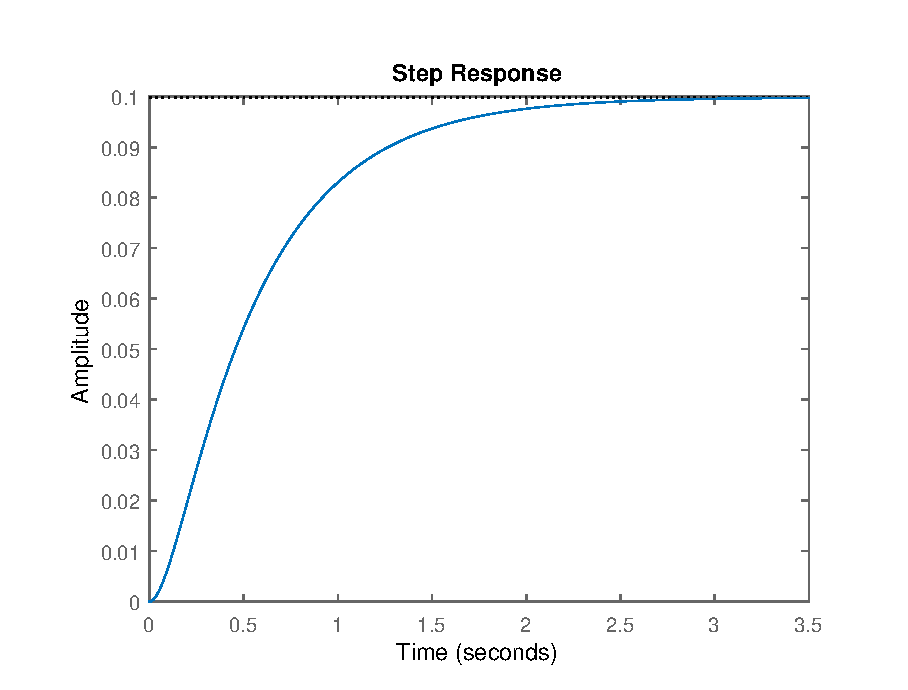
\includegraphics[width = 0.8\textwidth]{assets/image/UJI_SISTEM_2_1.eps}
                        \caption{Plot respon sistem dengan \textit{input step}}
                        \label{plot_respon_sistem_motor_1}
                    \end{figure}
                \subsubsection{Representasi sistem dalam bentuk \textit{state space}}
                    \lstinputlisting[language = matlab]{assets/code/REP_TF_SS.m}
                    \lstinputlisting[language = matlab]{assets/code/CONSOLE_REP_TF_SS.m}
                \subsubsection{Uji \textit{controllability} sistem}
                    \lstinputlisting[language = matlab]{assets/code/UJI_CRTB_SISTEM_2.m}
                    \lstinputlisting[language = matlab]{assets/code/CONSOLE_UJI_CRTB_SISTEM_2.m}
                \subsubsection{Perancangan Kendali Full State Feddback}
                    Perancangan kendali \textit{full state feedback} dengan parameter nilai \textit{overshoot} kurang dari $5$ persen (ditetapkan nilai \textit{overshoot} $ = 4.5\%$) dan nilai \textit{time settling} $2$ persen kurang dari $2$ detik (ditetapkan nilai \textit{time settling} $ = 1.5 detik$) dapat dilakukan dengan melakukan analisis secara matematis dengan persamaan \eqref{persamaan_13}. Pada persamaan \eqref{persamaan_13} terdapat nilai $\xi$ dan nilai $\omega_n$ yang digunakan untuk mencari \textit{pole} untuk memanipulasi karakteristik sistem sesuai dengan karakteristik yang dituju. Persamaan \eqref{persamaan_13} membutuhkan nilai $\xi$ yang dapat diperoleh dari analisis presentase \textit{overshoot} dan nilai $\omega_n$ dari analisis \textit{time settling}.
                    \begin{equation}
                        s_{1,2} = -\xi\omega_n \pm i \omega_n \sqrt{1-\xi^2}\\[5pt]
                        \label{persamaan_13}
                    \end{equation}
                    Persamaan \eqref{persamaan_14} menunjukkan analisis persentase \textit{overshoot} untuk memperoleh nilai $\xi$.
                    \begin{equation}
                        \begin{split}
                            \xi &= \ffrac{\left|ln\left(\frac{MP}{100}\right)\right|}{\sqrt{\pi^2+ln^2\left(\frac{MP}{100}\right)}} \\[5pt]
                            \xi &= \ffrac{\left|ln\left(\frac{4.5}{100}\right)\right|}{\sqrt{\pi^2+ln^2\left(\frac{4.5}{100}\right)}}\\[5pt]
                            \xi &= \ffrac{3.10}{\sqrt{9.85 + 9.61}} \\[5pt]
                            \xi &= 0.70
                            \label{persamaan_14}
                        \end{split}
                    \end{equation}
                    Persamaan \eqref{persamaan_15} menunjukkan analisis \textit{time settling} untuk memperoleh nilai $\omega_n$.
                    \begin{equation}
                        \begin{split}
                            t_{s(2\%)} &= \frac{4}{\xi\omega_n} \\[5pt]
                            1.5 &= \frac{4}{0.70\omega_n} \\[5pt]
                            \omega_n &= 3.80 \\[5pt]
                            \label{persamaan_15}
                        \end{split}
                    \end{equation}
                    Hasil analisis persamaan \eqref{persamaan_14} dan persamaan \eqref{persamaan_15} dapat digunakan untuk mencari nilai \textit{pole} untuk memanipulasi sistem sebagaimana yang ditunjukkan pada Persamaan \eqref{persamaan_16}. 
                    \begin{equation}
                        \begin{split}
                            s_{(1,2)} &= -(0.70)(3.80) \pm i (3.80) \sqrt{1 - 0.70^2}\\[5pt]
                            s_{(1,2)} &= - 2.66 \pm 3.80 \sqrt{0.51} i
                            \label{persamaan_16}
                        \end{split}
                    \end{equation}
                \subsubsection{Mencari nilai penguatan state feedback}
                    Nilai $K$ atau \textit{state feedback} dapat dicari menggunakan metode subtitusi atau dengan metode ackermann. Kode program berikut menunjukkan pengguaan kedua metode tersebut untuk mencari nilai $K$.
                    \lstinputlisting[language=matlab, firstline=32, lastline=37]{assets/code/LAT_2_SYSTEM.m}
                    \lstinputlisting[language=matlab, firstline=45, lastline=52]{assets/code/CONSOLE_LAT_2_SYSTEM.m}
                \subsubsection{Simulasi loop tertutup}
                    Berikut merupakan kode program untuk simulasi loop tertutup pada sistem,
                    \lstinputlisting[language=matlab, firstline=39, lastline=46]{assets/code/LAT_2_SYSTEM.m}
                    Grafik respon sistem ditunjukkan sebagai pada Gambar \ref{perbandingan_tuning}.
                    \begin{figure}[H]
                        \centering
                        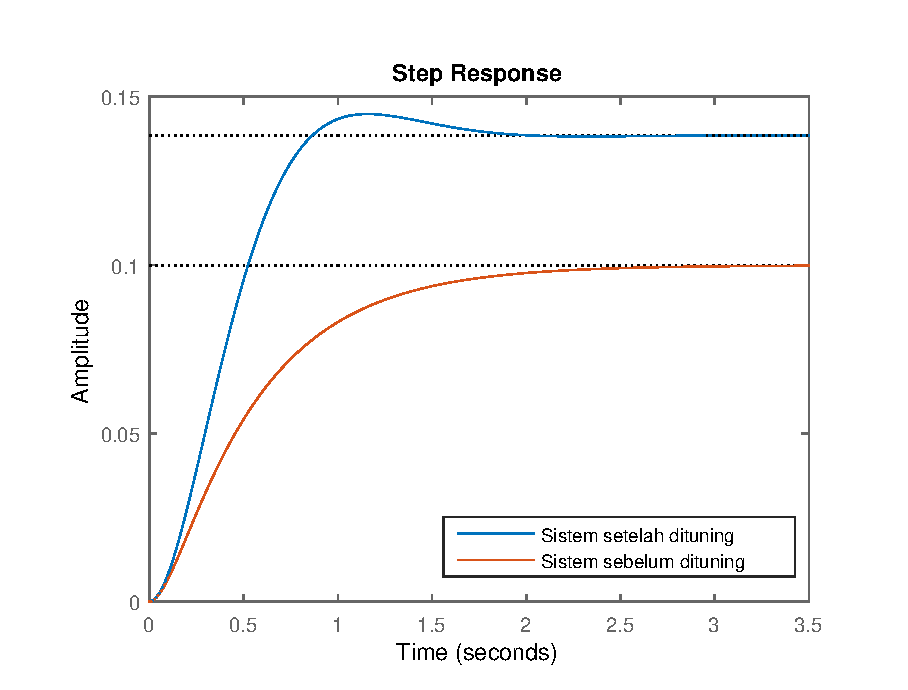
\includegraphics[width = 0.8\textwidth]{assets/image/UJI_SISTEM_2_3_rev.eps}
                        \caption{Plot perbandingan karakteristik sistem sebelum dilakukan \textit{tuning} dan setelah dilakukan \textit{tuning}}
                        \label{perbandingan_tuning}
                    \end{figure}
                \subsubsection{Perbandingan performa sistem}
                    Berikut merupakan kode program untuk membandingkan performa dari sistem sebelum dilakukan \textit{tuning} dan sistem sesudah dilakukan \textit{tuning},
                    \lstinputlisting[language=matlab, firstline=48, lastline=52]{assets/code/LAT_2_SYSTEM.m}
                    \textit{output} dari program diatas adalah nilai-nilai yang menunjukkan karakteristik dari sistem. Pada sistem yang telah dilakukan \textit{tuning} dapat diamati bahwa nilai nilai \textit{settling time} dan nilai \textit{overshoot} mendekati nilai yang telah ditetapkan $MP = 4.5\%$ dan \textit{time settling} $ = 1.5 detik$. Hasil ini telah sesuai dengan spesifikasi sistem yaitu nilai \textit{overshoot} kurang dari $5 persen$ dan nilai \textit{time settling} kurang dari $2 detik$.
                    \lstinputlisting[language=matlab, firstline=54, lastline=78]{assets/code/CONSOLE_LAT_2_SYSTEM.m}
    \section{Kesimpulan}
        Dari hasil percobaan dan pembahasan diatas, didapatkan kesimpulan sebagai berikut,
        \begin{enumerate}
            \item Letak pole berpengaruh pada karakteristik sistem, terdapat dua metode untuk memanupulasi letak pole yaitu metode subtitusi dan metode ackermann.
            \item Manipulasi letak pole pada sistem dapat dilakukan menggunakan parameter \textit{overshoot} dan parameter \textit{time settling}.
        \end{enumerate}
    \begin{thebibliography}{2}
        \bibitem[1]{Fahmizal} Fahmizal. 2020. "Pole Placement" dalam \textit{Modul Praktikum Teknik Kendali Lanjut} (hlm.1-4). Yogyakarta
    \end{thebibliography}
\end{document}